% 2013
% Maciej Szeptuch
% II UWr

\documentclass[11pt,leqno]{article}

\usepackage[utf8]{inputenc}
\usepackage{polski}
\usepackage{a4wide}
\usepackage[cm]{fullpage}

\usepackage{graphicx}
\usepackage{epstopdf}
\usepackage{amsmath,amssymb}
\usepackage{bm}
\usepackage{amsthm}

%% Kropka po numerze paragrafu, podparagrafu, itp.
\makeatletter
    \renewcommand\@seccntformat[1]{\csname the#1\endcsname.\quad}
    \renewcommand\numberline[1]{#1.\hskip0.7em}
\makeatother

%% Numeracja wzorów
\renewcommand{\theequation}{\arabic{section}.\arabic{equation}}

%%%%%%%%%%%%%%%%%%%%%%%%%%%%%%%%%%%%%%%%%%%%%%%%%%%%%%%%%%%%%%%%%%%%%%%%%%%%%%%%

\title{\LARGE \textbf{{Pracownia z analizy numerycznej}}\\
      {\Large Sprawozdanie do zadania \textbf{P3.5.}}\\
      {\large Prowadzący: dr Paweł Woźny}
}
\author{Maciej Szeptuch}
\date{Wrocław, \today}

\begin{document}
\thispagestyle{empty}
\maketitle

%%%%% WSTĘP
\section{Wstęp - całkowanie numeryczne}\label{S:Wstęp}
Pojęcie całki pojawia się w matematyce i fizyce bardzo często. W obliczaniu pól
figur płaskich, powierzchni brył obrotowych, czy z fizyki drogi punktu
materialnego w ruchu zmiennym lub liczeniu pracy stosuje się właśnie całki
oznaczone. Wyznaczanie dokładnej wartości całki z wykorzystaniem funkcji
pierwotnej jest w wielu przypadkach bardzo trudne. Szczególnie kiedy mamy do
czynienia z funkcjami, które nie są całkowalne elementarnie lub gdy, jak na
przykład w przypadku doświadczeń, mamy funkcję zdefiniowaną przy pomocy tablicy
wartości. W takich sytuacjach jesteśmy zmuszeni stosować metody umożliwiające
przybliżanie wartości całki. Takie metody nazywamy właśnie całkowaniem
numerycznym, inaczej kwadraturami. Główną ideą tych metod jest zastąpienie
funkcji podcałkowej inną funkcją, dla której obliczenie wartości całki jest
prostsze.

\subsection{Kwadratury interpolacyjne}\label{SS:KwadraturyInterpolacyjne}
Jedną z grup kwadratur są kwadratury interpolacyjne. Należą do niej metody,
w których przybliżamy funkcję podcałkową wielomianem interpolacyjnym zgodnie
z wzorem interpolacyjnym Lagrange'a.
$$
    p(x) = \sum_{i=0}^n f(x_i) \prod_{j=0 \and j \ne i}^n \frac{x - x_j}{x_i - x_j}
$$
Całkę z $f(x)$ możemy wtedy przybliżyć za pomocą wyrażenia
$$
    \int_a^b f(x) \mathrm{d}x \simeq \int_a^b p(x) \mathrm{d}x = \sum_{i=0}^n f(x_i) \int_a^b \prod_{j=0 \and j \ne i}^n \frac{x - x_j}{x_i - x_j} \mathrm{d}x
$$
Stosując te metodę przybliżenie jest lepsze, im wyższy jest stopień wielomianu
interpolacyjnego. W praktyce, z powodu błędów zaokrągleń itp., stosuje się
kwadratury złożone, w których dzieli się przedział całkowania na podprzedziały
i w nich stosuje się kwadraturę interpolacyjną niskiego stopnia, po czym sumuje
się otrzymane wyniki.

\newpage
\subsection{Metoda trapezów}\label{SS:MetodaTrapezow}
Jest to kwadratura interpolacyjna przy $n=1$, czyli stosując wielomian
pierwszego stopnia. Dla dwóch węzłów $x_0=a$ i $x_1=b$ otrzymujemy
$$
    \int_a^b f(x) \mathrm{d}x \simeq \frac{1}{2}(b - a)[f(a) + f(b)]
$$
Błąd wzoru trapezów wynosi
$$
    -\frac{1}{12}(b - a)^3f''(\xi) \qquad\mbox{(gdzie $\xi \in (a,b)$)}
$$
Dzieląc przedział całkowania na mniejsze poprzedziały i stosując wzór trapezów
dla każdego z nich otrzymamy tzw. złożony wzór trapezów
$$
    \int_a^b f(x)\mathrm{d}x \simeq \frac{1}{2}\sum_{i=1}^n (x_i - x_{i-1})[f(x_{i-1}) + f(x_i)]
$$

\subsection{Ekstrapolacja Richardsona}\label{SS:EkstrapolacjaRichardsona}
Esktrapolacja jest to prognozowanie wartości funkcji poza zakresem dla którego
mamy dane na podstawie dotychczas znanych wartości. Ekstrapolacja Richardsona
jest metodą uzywaną do przyspieszania zbieżności ciągu. Mając dany parametr $h$
niech $B(h)$ będzie przybliżeniem $A$ zależnym od $h$, takim o którym wiemy, że
$$
    A - B(h) = \sum_{i=0}^{\inf} a_ih^{b_i} \qquad\mbox{(gdzie $a_i$ są
    niewiadome, a $b_i$ są znane i wiemy, że $h^{b_i} > h^{b_{i+1}}$)}
$$
Wtedy możemy zapisać
$$
    A = B(h) + a_0h^{b_0} + O(h^{b_1})
$$
Biorąc powyższe równanie dla dwóch różnych wartości, np. $h$ oraz $h/2$,
otrzymujemy układ
$$
    A = B(h) + a_0h^{b_0} + O(h^{b_1})
$$
$$
    A = B(h/2) + a_0(h/2)^{b_0} + O(h^{b_1})
$$
Mnożąc drugie równanie przez $2^{b_0}$ i odejmując pierwsze otrzymujemy
$$
    (2^{b_0} - 1)A = 2^{b_0}B(h/2) - B(h) + O(h^{b_1})
$$
Z którego możemy wyliczyć A
$$
    A = \frac{2^{b_0}B(h/2) - B(h)}{2^{b_0} - 1} + O(h/{b_1})
$$
Teraz jeśli przyjmiemy za $C$
$$
    C = \frac{2^{b_0}B(h/2) - B(h)}{2^{b_0} - 1}
$$
Otrzymujemy lepsze przybliżenie A za pomocą C z błędem $O(h^{b_1})$.
Stosując tę metodę wiele razy, możemy otrzymywać coraz to lepsze przybliżenia
A.

\subsection{Metoda Romberga}\label{SS:MetodaRomberga}
Metoda całkowania numerycznego opierająca się na ekstrapolacji Richardsona oraz
wzorze trapezów. Polega ona na obliczaniu przybliżenia metodą trapezów dla
coraz mniejszych przedziałów oraz ekstrapolację wyników w celu uzyskania
mniejszych błędów - szybszej zbieżności. \\
Dzielimy przedział całkowania na $n=2^k$ równych przedziałów oraz konstruujemy
tzw. tablice Romberga $T_{m, k}$ (gdzie $m$ oznacza kolumnę a $k$ wiersz) za
pomocą wzorów
$$
    T_{0, k} = T_{2^k}(f) = h_k\sum_{i=0}^{2^k}'' f(x_i)
$$
oraz
$$
    T_{m, k} = \frac{4^mT_{m-1, k+1} - T_{m-1, k}}{4^m - 1}
$$

gdzie $h_k = (b - a) / 2^k$ i $x_i = a + ih_k$.
Pierwsza kolumna($T_{0, k}$) to zastosowanie wzoru trapezów, a następne to użycie
ekstrapolacji Richardsona w celu zmniejszenia błędu.

\subsection{Wariant metody Romberga}\label{SS:ZlozonaMetodaRomberga}
Metoda podana w zadaniu, zwana dalej \textit{złożoną} metodą Romberga, polega
na podzieleniu całki na mniejsze podprzedziały i obliczaniu metodą Romberga
przybliżeń na tych podprzedziałach przy warunku końcowym określonym przez
liczbę dokładnych cyfr pomiędzy obliczeniami kolejnych wierszy, maksymalną
liczbą wierszy równą $4$ oraz dostosowywaniu długości kolejnych podprzedziałów
w zależności od liczby wierszy w poprzednim kroku. Jeśli było to $1$ to
zwiększamy $h$, natomiast jeśli $4$ to zmniejszamy i powtarzamy obliczenie.

\section{Doświadczenie}\label{Doswiadczenie}
Korzystając z metody Romberga(\textbf{MR}) oraz \textit{złożonej} metody
Romberga(\textbf{ZMR}), obliczono przybliżenia 5 całek z dokładnością do 9 cyfr
dziesiętnych i na ich podstawie porównano skuteczność tych dwóch metod.
Skuteczność została określona na podstawie liczby wykonanych operacji
arytmetycznych, liczby wywołań funkcji podcałkowej (liczby węzłów) potrzebnych
do uzyskania przybliżenia oraz oczywiście uzyskanych wyników. Wartości dokładne
zostały uzyskane przy pomocy Wolframa\footnote{https://wolframalpha.com}.

\subsection{Całka $\int_{0}^{6}e^x\mathrm{d}x$}
\begin{center}\begin{figure}[ht]\begin{center}
    \caption{Funkcja $e^x$}
    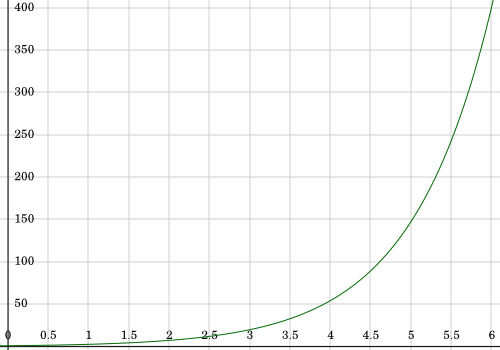
\includegraphics[scale=0.3,angle=0]{ex.png}
\end{center}\end{figure}\end{center}

\begin{center}\begin{table}[ht]\begin{center}
    \caption{Całka $\int_{0}^{6}e^x\mathrm{d}x$}
    \begin{tabular}{|c|l|c|c|c|} \hline
        \texttt{Metoda} & \texttt{Wynik}            & \texttt{Liczba węzłów} & \texttt{Liczba operacji arytmetycznych} & \texttt{h} \\ \hline
        Dokładny        & $\textbf{402.4287934927}$ &                        &                                         &            \\ \hline
        MR              & $\textbf{402.4287934927}$ & $\textbf{129}$         & $\textbf{1989}$                         &            \\ \hline
        ZMR             & $\textbf{402.4287934927}$ & $161$                  & $3384$                                  & $2.00$     \\ \hline
        ZMR             & $\textbf{402.4287934927}$ & $161$                  & $3102$                                  & $0.75$     \\ \hline
        ZMR             & $\textbf{402.4287934927}$ & $537$                  & $9581$                                  & $0.09$     \\ \hline
        ZMR             & $\textbf{402.4287934927}$ & $2401$                 & $40828$                                 & $0.01$     \\ \hline
    \end{tabular}
\end{center}\end{table}\end{center}

Wyniki działania obu algorytmów są identyczne, lecz złożona metoda w najlepszym
przypadku używa trochę więcej węzłów(około 25\%) dla długości przedziałów $2$
i $0.75$. Metodzie Romberga do wyznaczenia wartości całki jest potrzebne $129$
węzłów. Złożona metoda dla przedziału długości $0.01$ potrzebuje $2401$ węzłów,
dziewięciokrotne zwiększenie długości przedziału do $0.09$ skutkuje czterokrotnym
zmniejszenim liczby przedziałów do $537$. Następne ośmiokrotne zwiększenie -
przejście do długości $0.75$ daje już cztery razy mniejszą, najlepszą liczbę
węzłów dla tej metody - $161$, dalsze zwiększanie długości powoduje już
tylko występowanie nawrotów przez co zwiększa się jedynie liczba operacji
arytmetycznych a liczba węzłów pozostaje bez zmian.

\subsection{Całka $\int_{0}^{1}256x^9 - 576x^7 + 431x^5 - 120x^3 + 9x\mathrm{d}x$}
\begin{center}\begin{figure}[ht]\begin{center}
    \caption{Funkcja $256x^9 - 576x^7 + 431x^5 - 120x^3 + 9x$}
    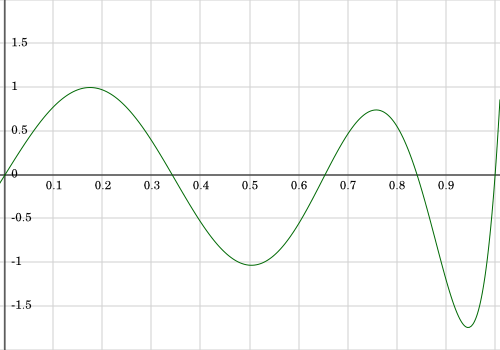
\includegraphics[scale=0.3,angle=0]{cheb.png}
\end{center}\end{figure}\end{center}
\begin{center}\begin{table}[ht]\begin{center}
    \caption{Całka $\int_{0}^{1}256x^9 - 576x^7 + 431x^5 - 120x^3 + 9x\mathrm{d}x$}
    \begin{tabular}{|c|l|c|c|c|} \hline
        \texttt{Metoda} & \texttt{Wynik}            & \texttt{Liczba węzłów} & \texttt{Liczba operacji arytmetycznych} & \texttt{h} \\ \hline
        Dokładny        & $\textbf{0.1000000000}$   &                        &                                         &            \\ \hline
        MR              & $\textbf{0.1000000000}$   & $\textbf{33}$          & $\textbf{542}$                          &            \\ \hline
        ZMR             & $\textbf{0.1000000000}$   & $129$                  & $3102$                                  & $1.00$     \\ \hline
        ZMR             & $\textbf{0.1000000000}$   & $129$                  & $2538$                                  & $0.25$     \\ \hline
        ZMR             & $\textbf{0.1000000000}$   & $137$                  & $2399$                                  & $0.12$     \\ \hline
        ZMR             & $\textbf{0.1000000000}$   & $493$                  & $8525$                                  & $0.01$     \\ \hline
    \end{tabular}
\end{center}\end{table}\end{center}

W tym przypadku również dostajemy poprawne, identyczne wyniki. Tak jak poprzednio
metoda Romberga radzi sobie najlepiej. Wystarczają jej $33$ węzły aby obliczyć
dokładną wartość. Złożona metoda w najlepszym wypadku potrzebuje około cztery
razy więcej, aż $129$ węzłów. Podobnie jak w poprzednim przypadku zaczynając od długości
$0.01$ zwiększając długość przedziału dwunastokrotnie do $0.12$ otrzymujemy
około cztery razy mniej węzłów - $137$, następne dwukrotne powiększenie do $0.25$
daje już tylko kilka węzłów mniej - $129$ po czym pogorsza się już tylko liczba
operacji arytmetycznych spowodowana nawrotami.

\newpage
\subsection{Całka $\int_{0}^{8}2 / (2 + \sin(\pi10x))\mathrm{d}x$}
\begin{center}\begin{figure}[ht]\begin{center}
    \caption{Funkcja $2 / (2 + \sin(\pi10x))$}
    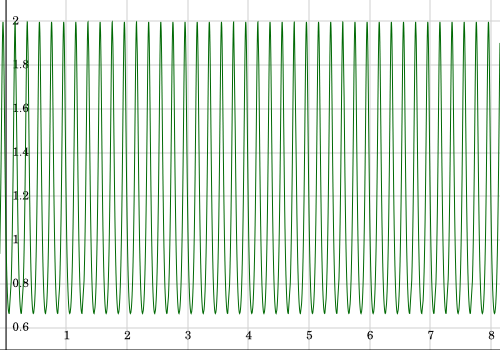
\includegraphics[scale=0.3,angle=0]{sinpi10x.png}
\end{center}\end{figure}\end{center}
\begin{center}\begin{table}[ht]\begin{center}
    \caption{Całka $\int_{0}^{8}2 / (2 + \sin(\pi10x))\mathrm{d}x$}
    \begin{tabular}{|c|l|c|c|c|} \hline
        \texttt{Metoda} & \texttt{Wynik}            & \texttt{Liczba węzłów} & \texttt{Liczba operacji arytmetycznych} & \texttt{h} \\ \hline
        Dokładny        & $\textbf{9.2376043072}$   &                        &                                         &            \\ \hline
        MR              & $8.0000000000$            & $3$                    & $28$                                    &            \\ \hline
        MR(10)          & $\textbf{9.237604307}8$   & $\textbf{1025}$        & $\textbf{14780}$                        &            \\ \hline
        ZMR             & $8.0000000000$            & $7$                    & $84$                                    & $2.00$     \\ \hline
        ZMR             & $\textbf{9.}0829037683$   & $5727$                 & $103797$                                & $1.00$     \\ \hline
        ZMR             & $\textbf{9.2376043072}$   & $6017$                 & $107692$                                & $0.25$     \\ \hline
    \end{tabular}
\end{center}\end{table}\end{center}

Ta całka sprawia probelmy zarówno zwykłej metodzie Romberga jak i
\textit{złożonej}. Z pomocą zwykłej metody otrzymujemy bezwartościowy wynik
$8$ którego obliczenie kosztowało nas za to tylko trzy węzły. \textit{Złożona}
metoda radzi już sobie lepiej, ale należy uważać z długością przedziału. Jeśli
początkowa wartość zostanie wybrana niefortunnie, również możemy otrzymać
niepoprawny wynik. Można to zauważyć dla przedziałów długości $2$ oraz $1$,
których wyniki to odpowiednio $8$ jak w przypadku zwykłego Romberga oraz
$9.0829...$, którego błąd wynosi około $0.2$. A oczekiwaliśmy dziewięciu
cyfr dziesiętnych poprawnych. Dla przedziału $0.25$ metoda daje już poprawny
wynik korzystając z $6017$ węzłów. Wartym zauważenia jest fakt, że wymuszenie
w zwykłym Rombergu obliczania co najmniej 10 wierszy pozwala uzyskać dokładny
wynik przy wykorzystaniu sześciokrotnie mniejszej liczby węzłów równej $1025$.
Pozwala to przypuszać, że w przypadkach gdy metoda Romberga daje niepoprawny
wynik opłacalnym jest obliczenie kilku wierszy więcej niż wykorzystywać do
obliczeń drugi wariant.

\subsection{Całka $\int_{0.02}^{0.2}\sin(\frac{1}{x})\mathrm{d}x$}
\begin{center}\begin{figure}[ht]\begin{center}
    \caption{Funkcja $\sin(\frac{1}{x})$}
    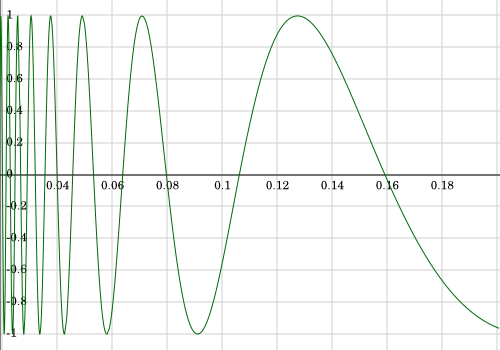
\includegraphics[scale=0.3,angle=0]{sindivx.png}
\end{center}\end{figure}\end{center}
\begin{center}\begin{table}[ht]\begin{center}
    \caption{Całka $\int_{0.02}^{0.2}\sin(\frac{1}{x})\mathrm{d}x$}
    \begin{tabular}{|c|l|c|c|c|} \hline
        \texttt{Metoda} & \texttt{Wynik}            & \texttt{Liczba węzłów} & \texttt{Liczba operacji arytmetycznych} & \texttt{h} \\ \hline
        Dokładny        & $\textbf{-0.0021359945}$  &                        &                                         &            \\ \hline
        MR              & $\textbf{-0.0021359945}$  & $4097$                 & $58026$                                 &            \\ \hline
        ZMR             & $\textbf{-0.0021359945}$  & $\textbf{778}$         & $15524$                                 & $0.18$     \\ \hline
        ZMR             & $\textbf{-0.0021359945}$  & $\textbf{778}$         & $\textbf{15242}$                        & $0.09$     \\ \hline
        ZMR             & $\textbf{-0.0021359945}$  & $993$                  & $18514$                                 & $0.03$     \\ \hline
        ZMR             & $\textbf{-0.0021359945}$  & $825$                  & $15176$                                 & $0.01$     \\ \hline
    \end{tabular}
\end{center}\end{table}\end{center}

Ta całka sprawiła problem już tylko metodzie Romberga. Obie metody dały
identyczny, poprawny wynik, ale zwykła potrzebowała do obliczeń $4097$ węzłów,
podczas gdy \textit{złożonej} w najlepszym przypadku wystarcza ponad pięć razy
mniej - $778$ węzłów. Dla przedziału długości $0.01$ potrzebuje ona $825$
węzłów zwiększenie długości przedziału do $0.03$ sprawia, że potrzebuje ona
więcej bo $993$ węzły. Przy następnym zwiększeniu długości sytuacja się
poprawia i zapotrzebowanie na węzły spada do $778$. Dalsze zwiększanie długości
powoduje już tylko występowanie nawrotów, a co za tym idzie zwiększenie liczby
operacji arytmetycznych. Tutaj możemy zauważyć, że nie zawsze zmniejszenie
długości przedziałów powoduje zwiększenie liczby węzłów, czasem może wystąpić
przeciwna sytuacja.

\subsection{Całka $\int_{0}^{7}\frac{1}{1 + x^4}\mathrm{d}x$}
\begin{center}\begin{figure}[ht]\begin{center}
    \caption{Funkcja $\frac{1}{1 + x^4}$}
    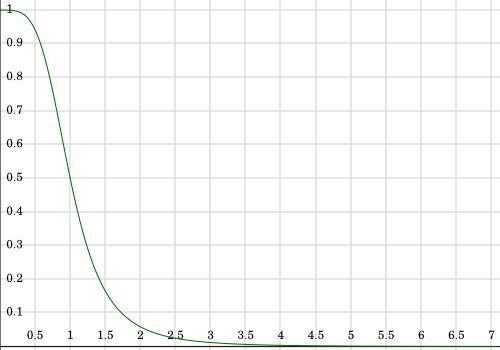
\includegraphics[scale=0.3,angle=0]{poly.png}
\end{center}\end{figure}\end{center}
\begin{center}\begin{table}[ht]\begin{center}
    \caption{Całka $\int_{0}^{7}\frac{1}{1 + x^4}\mathrm{d}x$}
    \begin{tabular}{|c|l|c|c|c|} \hline
        \texttt{Metoda} & \texttt{Wynik}            & \texttt{Liczba węzłów} & \texttt{Liczba operacji arytmetycznych} & \texttt{h} \\ \hline
        Dokładny        & $\textbf{1.1097490907}$   &                        &                                         &            \\ \hline
        MR              & $\textbf{1.1097490907}$   & $513$                  & $7516$                                  &            \\ \hline
        ZMR             & $\textbf{1.1097490907}$   & $\textbf{245}$         & $5148$                                  & $2.00$     \\ \hline
        ZMR             & $\textbf{1.1097490907}$   & $\textbf{245}$         & $\textbf{4302}$                         & $0.25$     \\ \hline
        ZMR             & $\textbf{1.1097490907}$   & $421$                  & $7329$                                  & $0.09$     \\ \hline
        ZMR             & $\textbf{1.1097490907}$   & $1483$                 & $25164$                                 & $0.01$     \\ \hline
    \end{tabular}
\end{center}\end{table}\end{center}

Wyniki obu metod są idenyczne. W tym przypadku metoda Romberga też potrzebuje
większej liczby węzłów, ale nie tak bardzo jak poprzednio. Do obliczenia wyniku
potrzebowała ona $513$ węzłów, natomiast \textit{złożonej} w najlepszym wypadku
wystarcza tylko $245$ węzłów. Dla długości $0.01$ \textit{złożona} metoda
Romberga wykorzystuje $1483$ węzły, dziewięciokrotne wydłużenie przedziału do
$0.09$ pozwala zmniejszyć liczbę węzłów do $421$. Następne zwiększenie długości
do $0.25$ sprawia, że wykorzystuje ona już tylko $245$, dalsze zwiększanie
skutkuje już tylko zwiększeniem liczby operacji arytmetycznych.

\section{Wnioski}\label{S:Wnioski}
Jak możemy zauważyć na podstawie wykonanych doświadczeń, \textit{złożona}
metoda Romberga, uwzględniająca charakter zmienności funkcji, jest algorytmem,
którego stosowanie w niektórych przypadkach jest dobrym rozwiązaniem. Dobrze radzi
sobie ona np. z niektórymi funkcjami okresowymi - przy odpowiednim doborze
początkowej długości przedziału - w przypadku których zwykła metoda Romberga może mieć
kłopot z obliczeniem poprawnego wyniku. Jednakże w takich przypadkach jest możliwe,
że ustalenie minimalnej liczby wierszy w zwykłym Rombergu pozwoli otrzymać lepsze
rezultaty. W ogólności nie ma jednoznacznego określenia, która wersja jest lepsza,
przy wyborze metody bardzo ważnym jest zwracanie uwagi na szczególne własności
obliczanych całek.

\thispagestyle{empty}
\begin{thebibliography}{99}
    \bibitem{Not} S. Lewanowicz, \textit{Notatki do wykładu z analizy numerycznej}, Wrocław, 2012r.
    \bibitem{Kin} D. Kincaid, W. Cheney \textit{Analiza Numeryczna}, Wydawnictwa Naukowo-Techniczne, Warszawa 2006r.
    \bibitem{Wolfram} WolframAlpha, https://www.wolframalpha.com.
    \bibitem{Wikipedia} Wikipedia, https://en.wikipedia.org/wiki/Romberg\%27s\_method, \\https://en.wikipedia.org/wiki/Richardson\_extrapolation, https://en.wikipedia.org/wiki/Numerical\_integration
\end{thebibliography}
\end{document}
